\documentclass[runningheads]{llncs}
%
\usepackage[T1]{fontenc}
% Other packages included here
\usepackage{graphicx}
 \graphicspath{ {./Figures/} }
\usepackage{enumitem}
\usepackage{pgfplots}
\usepackage{pgf-pie}
\usepackage{doi}
\usetikzlibrary{patterns}
\pgfplotsset{compat=1.18}
%
% If you use the hyperref package, please uncomment the following two lines
% to display URLs in blue roman font according to Springer's eBook style:
%\usepackage{color}
%\renewcommand\UrlFont{\color{blue}\rmfamily}
%
\begin{document}
%
\title{AI Chatbot for mental health status detection using deep learning}
%
\author{Aditya Dilip Pansare\inst{1*} \and
Amrut Wali\inst{1} \and
Shresta U\inst{1} \and
Revanth RM\inst{1} \and
Farhana Kausar\inst{1}}
%
\institute{Atria Institute of Technology, Bangalore, Karnataka, India \\
\email{adi10pansare@gmail.com}}
%
\maketitle
%
\begin{abstract}
The paper aims to solve the problem of increasing depression and suicide rates in the recent years by making use of an IDPT(Interned Delivered Psychological Treatment) system, which is a self-administered recovery from depression by analyzing its presence online. This system employs a chat-bot which takes text input from a user to emulate a normal conversation. The text obtained is then passed on to a deep learning model which makes use of Word Vectorization method to create a model that is most efficient to classify text data into two classes namely Depressed and Non-Depressed categories. The model Is trained using the Distress Analysis Interview Corpus(DAIC-WOZ) dataset. The word vector is created using the Global Vectors for word representation(GloVe) machine learning model. The accuracy obtained is $65.79\%$. The model accuracy is comparatively less due to the very small amount of training data available.

\keywords{Chat-bot, Suicide, Depression, Self-administered, Word vectorization, GloVe}
\end{abstract}
%
\section{Introduction}
This research paper aims to solve the crisis of drastically increasing suicide rates. It has been determined that the major precursor to suicide is depression. Most of the time the person who is depressed does not even realize his condition and ignore all the symptoms until he will try to suicide. To prevent this we have proposed an internet delivered treatment method which can be used online by anyone to check their depression levels.

The model is an Interface of a chatbot which converses with the user like any normal human beings and asks questions. The data typed by the user is stored after each conversation. This data is then preprocessed and sent to the model.

The preprocessed data is then vectorized. This vector stores the data of similar words. Then the model analyzes this text against the trained data. A prediction score is generated which is fro $0$ to $100$.

This prediction will be an indicator of the percentage of depression a person currently has.
\section{Related Works}
 
\section{Methodology}
The whole system is made using the following steps: 

\subsection{Dataset Acquisition}
The dataset used is the DAIC WOZ dataset. This database contains clinical interviews designed to support the diagnosis of psychological distress conditions such as anxiety, depression, and post-traumatic stress disorder.

These interviews were collected as part of a larger effort to create a computer agent that interviews people and identifies verbal and nonverbal indicators of mental illness (DeVault et al., 2014). 

Data collected include audio and video recordings and extensive questionnaire responses; this part of the corpus includes data from the Wizard-of-Oz interviews, conducted by an animated virtual interviewer called Ellie, controlled by a human interviewer in another room.

Data has been transcribed and annotated for a variety of verbal and non-verbal features. This download includes 189 sessions of interactions ranging between 7-33 minutes (average is 16 minutes). Each session includes transcripts of the interaction, participant audio files, and information about facial features.

The dataset we are using will only be the transcripts text data. The dataset contains the features participant ID, start time, end time, speaker, speech.

Each file has two participants listed which is the AI which asks questions 'Ellie' and the other is the 'Participant' itself.

There is another file which has the participant depression indicator against his ID. It also has the PHQ8 score of each participant. But we will only be using the Boolean depression presence in our model.

\subsection{Data preprocessing}
We preprocess the data normally to remove all the unnecessary text data. We remove the start and end times. We remove each row where ellie speaks. and we will keep only the rows where the particpant speaks. The speech text data will only be retained.

The data processed now will be merged with the depression boolean indicator. Also the stop words are removed in all the text, and any missing data is discarded.

This is the dataset which is finally going to be used for training

\subsection{Model}

\begin{figure}[!ht]
\centering
\fbox{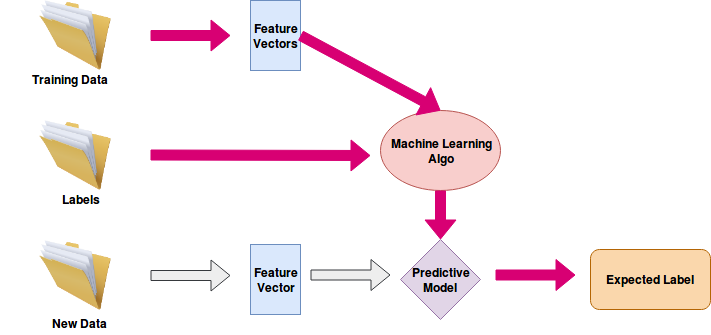
\includegraphics[width=\textwidth]{workflow.png}}
\caption{Workflow Diagram}
\label{figure:workflow}
\end{figure}
\section{Analysis}

\section{Conclusions}
In this paper we aimed to find a method to provide online assessment and treatment method for Depressive Disorders through the means of a chatbot. Various methods were studied on analysis of text and determination of severity of depression. 

The portions of the text that reflect the depressive behaviour of the person can be extracted using sentiment analysis and the severity  can be determined using neural network algorithms and mapping the result against clinical depression scale. 

These methods are the most feasible approach to create an AI based chatbot to detect and treat depression. The goal is to detect and cure Early signs of depression or Depressive Disorders in order to prevent suicide which is going to be the final stage.

% Bibliography
\bibliographystyle{splncs04}
\bibliography{References}

\end{document}